\documentclass[english]{article}
% a4 is the paper size
% english is for the language used in standard texts (figures, tables etc)
% twoside for doublesided pages. Remove if that is not wanted.

% ---------------------------------------------------------------------------- %
% Load base preamble
% ---------------------------------------------------------------------------- %

%Import from absolute path
%\usepackage{import}
%\import{C:/GitHub/LaTeX_Preamble_and_Examples/preamble/}{preamble_dk.tex}

%Import from a relative path
\usepackage{import}
\subimport{../preamble/}{preamble_en.tex}

% ---------------------------------------------------------------------------- %
% Local macros
% ---------------------------------------------------------------------------- %

% It is quite common that you are going to write the same thing multiple times.
% As part of the preamble I have predefined some macros for what I keep on
% having to use, and while I endorse you send a pull request with more, here you
% can add the ones you only need for this one document.

\newcommand{\PARTITION}{\textsc{PARTITION}}

% You can also define local macros here, that are used later in other files read
% using \input.
\newcommand{\Gmul}{\ensuremath{\calG_{\mathrm{mul}}}}

% ---------------------------------------------------------------------------- %
% Page layout
% ---------------------------------------------------------------------------- %
\usepackage[a4paper]{geometry}

% ---------------------------------------------------------------------------- %
% Bibliography
% ---------------------------------------------------------------------------- %
\usepackage[
  backend=biber,
  style=alphabetic, % options: alphabetic, numeric, ...
  sortlocale=EN_GB,
  useprefix=false,
  url=false,
  doi=true,
  eprint=false,
  maxbibnames=99,
]{biblatex}
\addbibresource{references.bib}


% Change the Bibliography to correctly handle Dutch names.
\renewbibmacro*{begentry}{\midsentence}

\makeatletter
\AtBeginDocument{\toggletrue{blx@useprefix}}
\AtBeginBibliography{\toggletrue{blx@useprefix}}
\makeatother


% ---------------------------------------------------------------------------- %
% Title
% ---------------------------------------------------------------------------- %
\newcommand{\coursename}{Course name}
\newcommand{\handinname}{Handin name}

% Font sizes of relevance: \normalsize, \large, \Large, \LARGE, \huge, \Huge
\title{{\LARGE Reverse engineerable \LaTeX examples}}

\author{Steffan Sølvsten\footnote{Together with numerous many other beautiful
    people at Aarhus Univesity.}}
\affil{Aarhus University \\ \mailto{soelvsten@cs.au.dk}}

\begin{document}

% Define title and more on frontpage
\maketitle

\begin{abstract}
  This document is created with the intention to make the learning curve of
  switching to \LaTeX\ simpler. It does this by giving an example or two of all
  types of writing usually done as part of a handin, such as math, code, proofs
  and much more. The code for all examples is made as easy to read as possible.
\end{abstract}

\newpage
\tableofcontents

\newpage
\section{Math} \label{sec:math}
Most basically you use \emph{equation} to write a mathematical equation on a
single new and centered line, such as the following
\begin{equation}
  x = y
\end{equation}
You can write math in the text by writing \$ x\_0 \$ = $x_0$. If you want to
write math over more lines, it is better to use the \emph{align} or even better
the \emph{alignat} commands. You can also use the * in the
$\backslash$\code{begin}$\{$\code{align}$\}$ to not include line numbers
\begin{align*}
  (R' \circ R)^{-1}
    &= (\{(a,b) \in S \times U | \exists t \in T: (a,t) \in R \wedge (t,b) \in R'\})^{-1}
\\
    &= \{(p,q) \in U \times S | (q,p) \in R \circ R' \}
\\
    &= \{(p,q) \in U \times S | \exists t \in T : (p,t) \in R'^{-1} \wedge (t,q) \in R^{-1}\}
\\
    &= R'^{-1} \circ R^{-1}
\end{align*}
In the following example with \emph{alignat}, we get the ability to have
multiple alignments in the same column, such that both the arrows on the left
and the equals sign are aligned nicely. Here is a reference to line
\ref{alignatL2}.
\begin{alignat}{2}
    && \cos x &= \cos x * \cos y \label{alignatL1}
\\ \ArrowBetweenLines
    && 0 &= \cos x * \cos y - \cos x \label{alignatL2}
\\ \ArrowBetweenLines
    && 0 &= \cos x \cdot (\cos y - 1) \label{alignatL3}
\end{alignat}

\subsection{Math fonts and symbols}
In mathmode you can also use different styles called alphabets. Bold
$\mathbf{b}$ and italic text such as functions can be written with
$\mathit{function}$. Finally with \emph{mathcal} you can get calligraphic
writing, such as $\mathcal{G}$ and with \emph{mathbb} you get math symbols for
fields, like $\mathbb{F}$, and other things such as $\mathbb{0}$.

Furthermore there are quite a few symbols are you normally have to write, such
as the real numbers $\mathbb{R}$. Hence, the preamble defines multiple shortcuts
in \emph{math\_macros\_symb} for \C, \Q, \F\ and many more. All these macros
ensure to go into math mode, so you will not get any compile errors in plain
writing. The file is easy to read and is well documented.

In general you would like to define macros for whenever you are going to reuse
the same notation over and over again. For example if you have to write about
the \cNP-complete problem \PARTITION\ multiple times, you may want to define
\PARTITION\ as a local macro, since it is not part of the preamble.

\subsection{Linear Algebra}
With \emph{pmatrix} matrices can also be made, such as in the following. For the
row operations I have made the \emph{ero} macro to make life easier.
\begin{equation*}
  \begin{pmatrix}[cc|c]
    2 & 1 & 1
    \\
    1 & 1 & 0
  \end{pmatrix}
  \ero{R_1 - R_2}{2R2}
  \begin{pmatrix}[cc|c]
    1 & 0 & 1
    \\
    2 & 2 & 0
  \end{pmatrix}
\end{equation*}

Other common (Linear) Algebra operators that I have made macros for are
$\Det{A}$, the equivalence class $\eqclass{v}{\calV}$, the matrix representation
$\matrep{\calV}{L}{\calW}$, the $\sgn{\sigma}$ and the $\Span{\seq{v}{1}{n}}$
can be made easily with the macros coded. The vectors \allones\ and \allzeros\
also have a shortcut.

\subsection{How to easily find symbols}
One good place to find the \LaTeX\ command for a symbol is at \http{detexify.kirelabs.org/classify.html}.

\subsection{Other math macros}
Things like sequences and sets we use all the time too, which is why I've made
macros. For a sequence you can write $\seq{a}{1}{n}{2}$ and for sets $ \set{x
  \in \Sigma^*}{ |x| \geq 42 } $. Both of these shortcuts are overloaded, such
that they can take fewer arguments than currently shown here.

% \newpage
\section{Proofs}
With logic and more you want to make a \emph{theorem}, \emph{lemma},
\emph{proposition}, \emph{corollary} or \emph{conjecture} followed possibly by a
\emph{proof}. These are all currently implemented in the localized preamble to
associate the same command to both languages. The lemma below has a label, which
is \ref{lem:Martin2_11} and can be used to reference it.

\begin{lemma}[Martin 2.11] \label{lem:Martin2_11}
  $\forall x \in \Sigma^* \forall (p,q) \in Q :
  \delta^* ((p,q),x) = (\delta_1^* (p,x) , \delta_2^* (q,x))$
\end{lemma}
\begin{proof}
  We prove this by induction in the construction of $x$.

  In the base case of $x$ being the empty string $\Lambda$
  \begin{align*}
    \delta^*((p,q), \Lambda) &= (p,q)
    &\text{def. 2.12}
    \\
                             &= (\delta_1^* (p,\Lambda) , \delta_2^* (q,\Lambda))
    &\text{def. 2.12}
  \end{align*}

  Now assume per induction that for $y \in \Sigma^*$ we have that
  $\delta^*((p,q), y) = (\delta_1^*(p,y), \delta_2^*(q,y))$ and consider $x = y
  \sigma$ for $\sigma \in \Sigma$.
  \begin{align*}
    \delta^*((p,q),y\sigma) &= \delta(\delta^*((p,q),y),\sigma)
    &\text{def. 2.12}
    \\
                            &= \delta((\delta_1^*(p,y), \delta_2^*(q,y)),\sigma)
    &\text{I.H.}
    \\
                            &= (\delta_1(\delta_1^*(p,y),\sigma), \delta_2(\delta_2^*(q,y),\sigma))
    &\text{def. af } \delta
    \\
                            &= (\delta_1^*(p,y\sigma), \delta_2^*(q,y\sigma))
    &\text{def. 2.12}
  \end{align*}
\end{proof}

\section{Formal proofs}

\subsection{proof trees}
The \texttt{bussproof} package allows to create proof trees. Usually this is
done with the command \emph{prooftree}. To not have an immediate line break
after, then the preamble also defines the environment \emph{bprooftree} that can
be used as shown in Figure~\ref{fig:bprooftree}.

\begin{figure}[ht!]
  \centering
  \begin{bprooftree}
    \AxiomC{\phantom{M}}
    \RightLabel{\scriptsize (MLeaf)}
    \UnaryInfC{\code{leaf} $\sim =\sim$ \code{leaf}}
  \end{bprooftree}
  \hspace{10pt} % add some spacing between the two proof trees
  \begin{bprooftree}
    \AxiomC{$c_1 \sim =\sim c_1'$}
    \AxiomC{$c_2 \sim =\sim c_2'$}
    \RightLabel{\scriptsize (MNode)}
    \BinaryInfC{\code{node} $c_1$ $x$ $c_2$ $\sim =\sim$ \code{node} $c_1'$ $x'$ $c_2'$}
  \end{bprooftree}
  \caption{Inductive relation for trees of the same shape}
  \label{fig:bprooftree}
\end{figure}

\subsection{logic proofs}
There exists various packages to make logic proofs, but after some time looking
around I've chosen to focus on the \emph{lplfitch} package, since its output
seems to be the generally preferred and used style. This package is very easy to
work with, when first learned, but until then you need to learn quite a lot of
new syntax. Most importantly notice, that a proof and subproof has two
arguments, the assumption and the conclusions.
\begin{center}
    \fitchprf{\pline[1.]{presumption}}{
        \pline[2.]{conclussion}
    \\  \subproof{\pline[3.]{assumption}}{
            \pline[4.]{conclussion}[argument]
        \\  \pline[5.]{conclussion}
        }
        \pline[6.]{conclussion}
    }
\end{center}

All the commands can be found in the documentation
\href{http://mirrors.dotsrc.org/ctan/macros/latex/contrib/lplfitch/lplfitch.pdf}{\emph{here}},
but most shortcuts are of the form: $"l" + type + "i/e"$. Argumentation is also
done using these shortcuts, so every line is
\begin{equation*}
    \backslash pline[\text{linenumber}]\{\text{formula}\}[\text{justification}]
\end{equation*}

Notice, that in fitch-style there isn't normally written assumption or premise,
but it is merely shown by the horizontal line. You can write it if you want. The
proof to exercise $1.2.1$ c from TØ class is in the proof to lemma
\ref{lem:121}.
\begin{lemma} \label{lem:121}
    $(p \wedge q) \wedge r \vdash p \wedge (q \wedge r)$
\end{lemma}
\begin{proof}
    \fitchprf{\pline[1.]{(p \land q) \land r}[\textbf{Premise}]}{
        \pline[2.]{r}[\lande{1}]
    \\  \pline[3.]{p \land q}[\lande{1}]
    \\  \pline[4.]{p}[\lande{3}]
    \\  \pline[5.]{q}[\lande{3}]
    \\  \pline[6.]{q \land r}[\landi{2, 5}]
    \\  \pline[7.]{p \land (q \land r)}[\landi{4, 6}]
    } \\ %Linebreak for the tombstone
\end{proof}

If you need a fresh variable, you don't create a subproof, but instead a boxed
subproof. Parts of the solution to an exercise in one of the handins is then
\begin{theorem} \label{thm:handin}
    $\forall x (P(x) \rightarrow Q(x) \vdash (\forall x \neg Q(x)) \rightarrow (\forall x \neg P(x)))$
\end{theorem}
\begin{proof}
    \fitchprf{
        \pline[1.]{...}}{
            \boxedsubproof[2.]{x_0}{\lnot Q(x_0)}{
                \pline[3.]{...}
            }
            \pline[4.]{...}
        } \\ %Linebreak for the tombstone
\end{proof}

\section{Tables and figures}
\begin{figure}[ht!] % h = Here, t = Top, b = Bottom, p = same Page, ! = DO AS I SAY
  \centering

  \begin{subfigure}{0.59\linewidth}
    \centering
    
    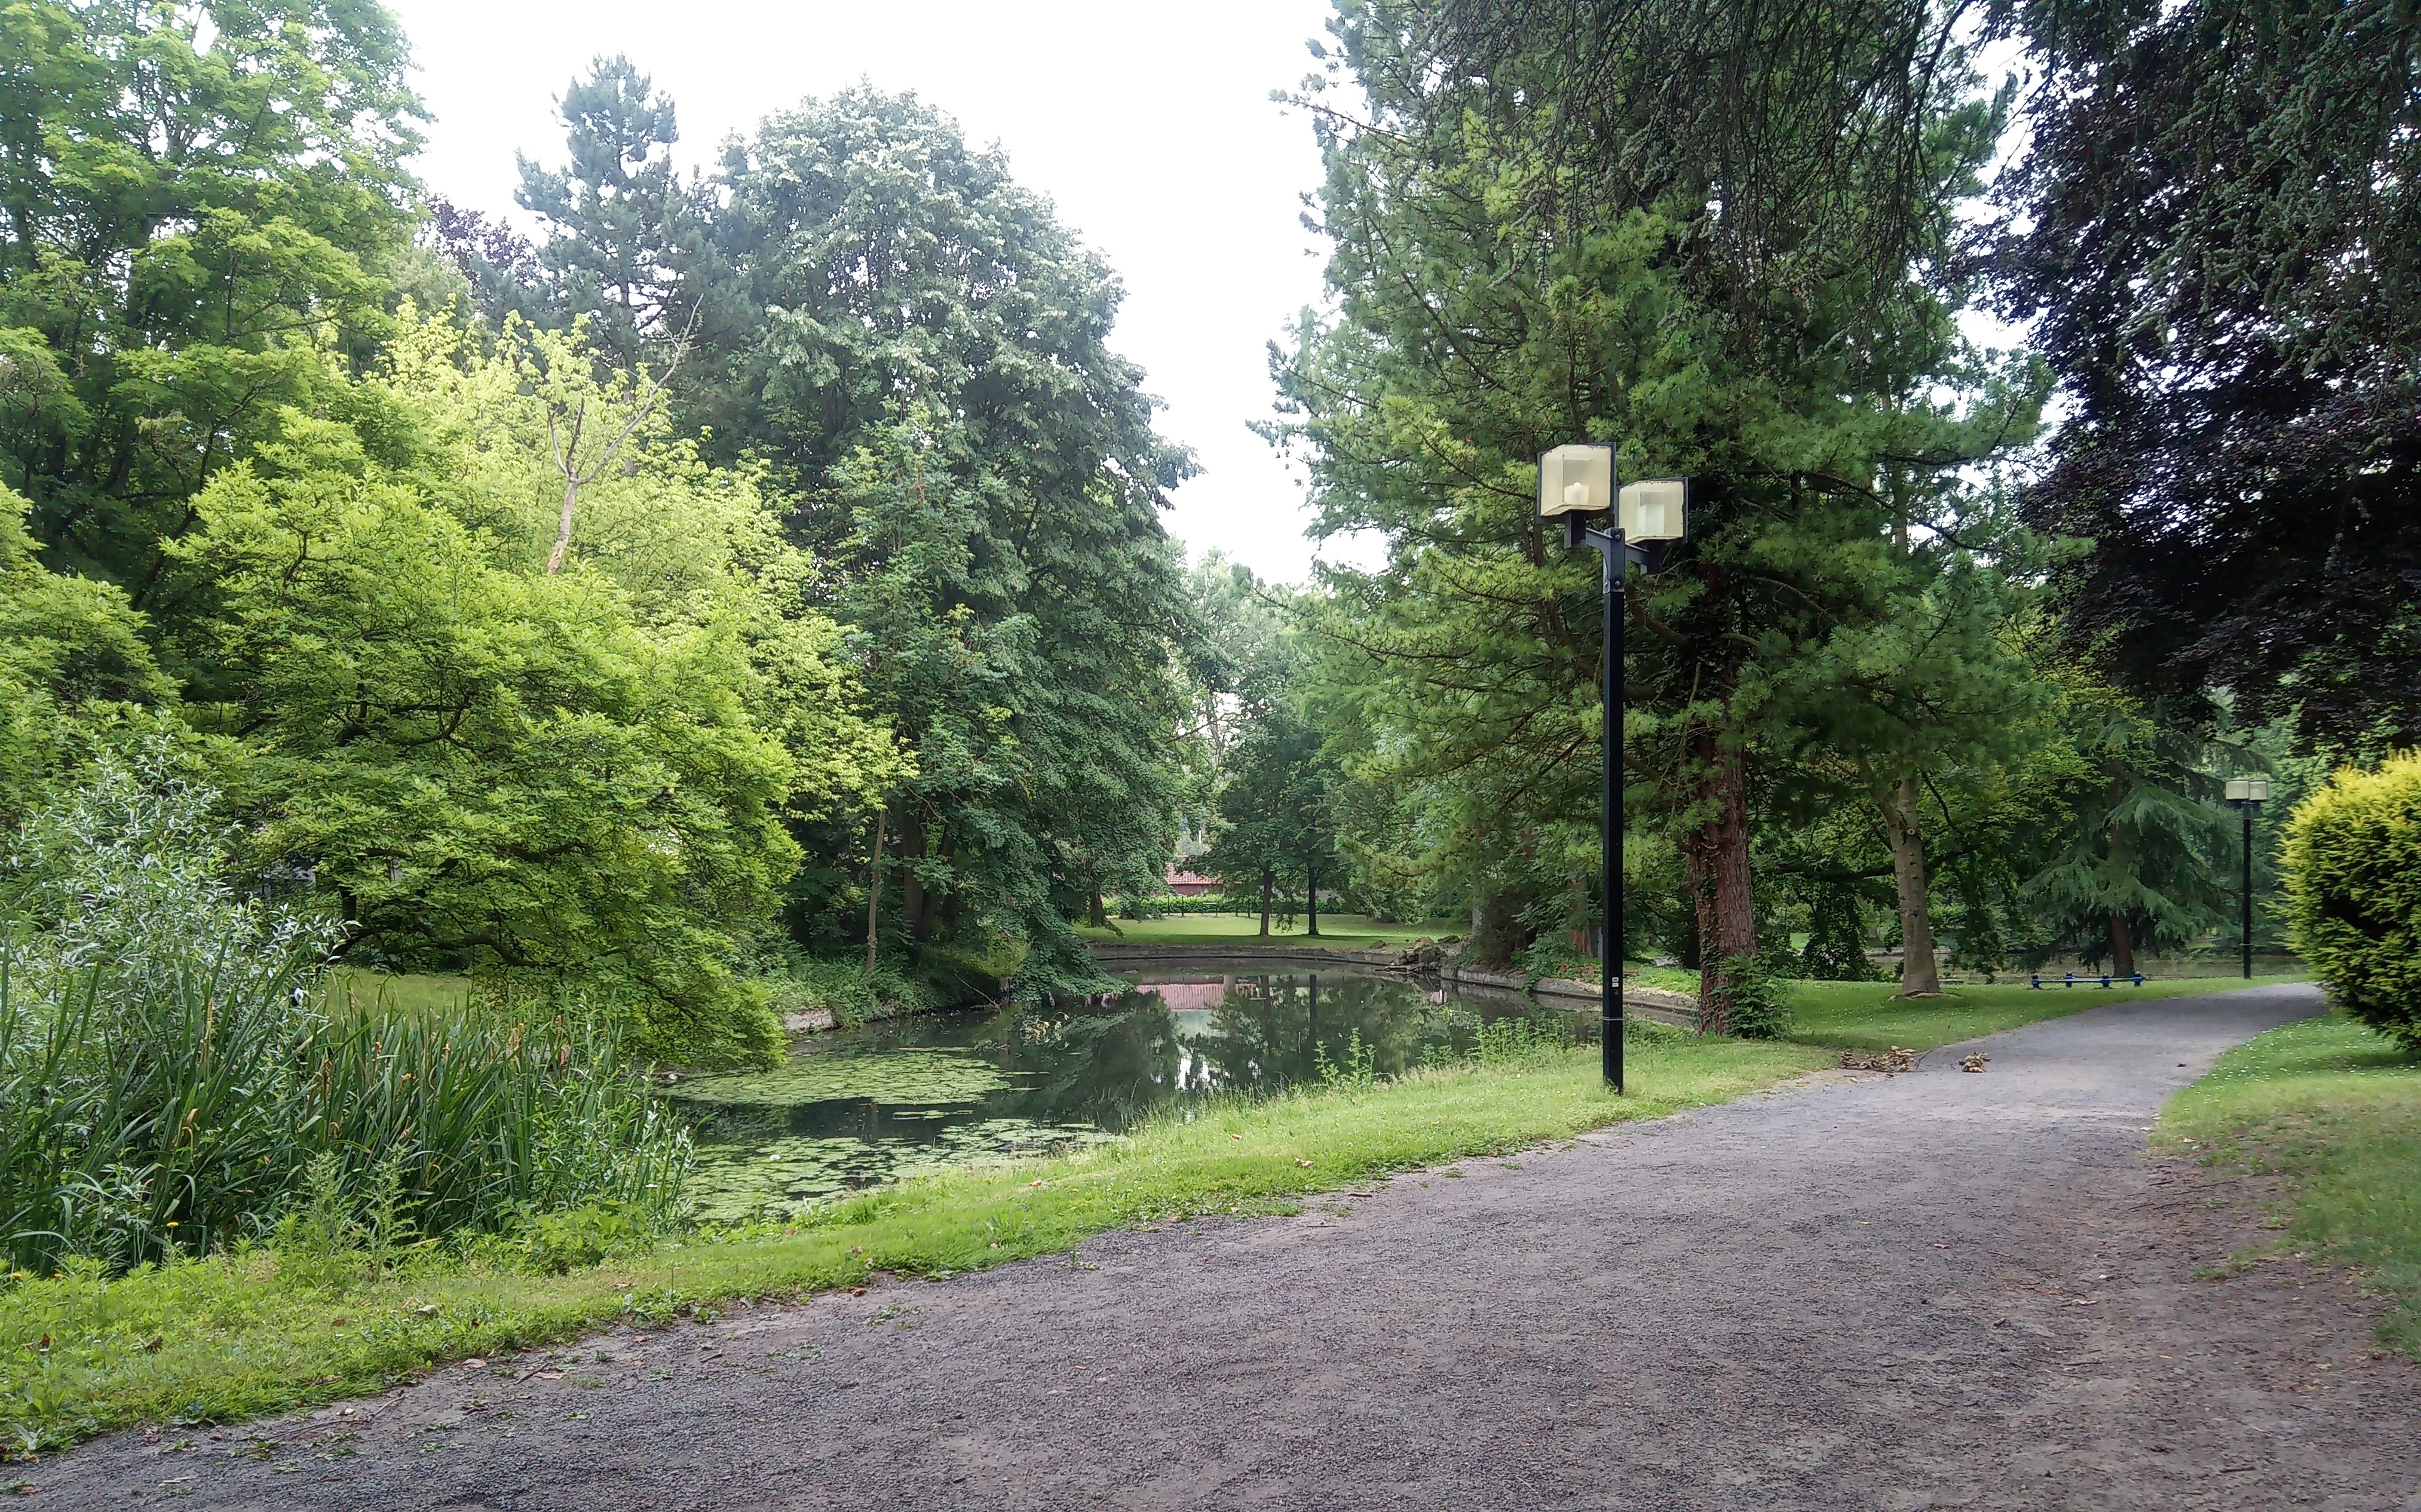
\includegraphics[width=\linewidth]{img/picture_1.jpg}
    
    \caption{An image}
    \label{fig example: sub figure 1}
  \end{subfigure}
  \begin{subfigure}{0.39\linewidth}
    \centering
    
    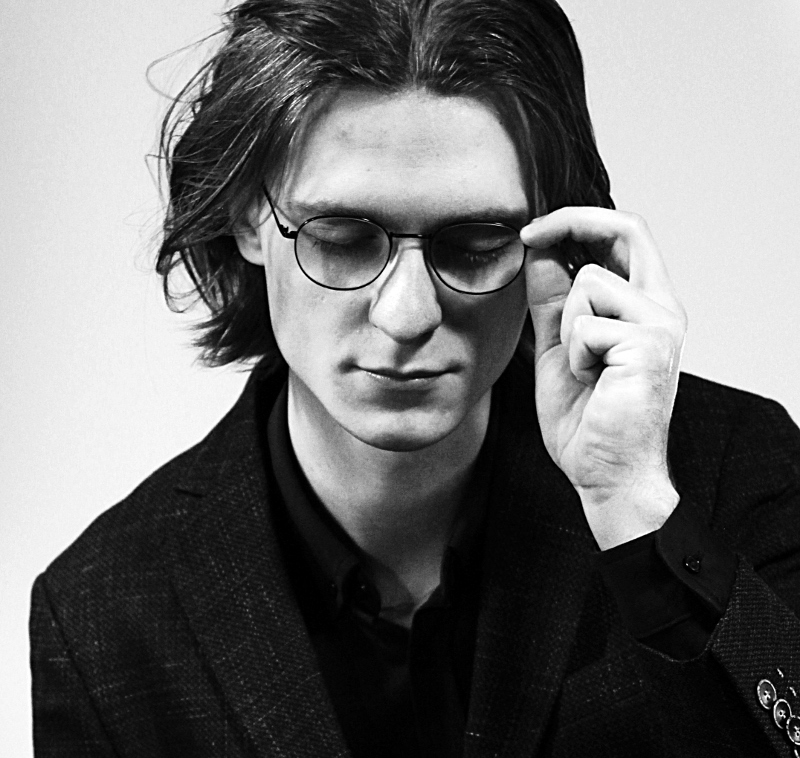
\includegraphics[width=\linewidth]{img/picture_2.jpg}
    
    \caption{Another image}
    \label{fig example: sub figure 2}
  \end{subfigure}


  \caption{Some pictures in subfigures}
  \label{FigExample}
\end{figure}

\begin{wrapfigure}[7]{r}{15em}
  \centering
  \begin{tikzpicture}[shorten >= 1, node distance = 2cm, on grid, auto]
    \node[shape = circle, draw = black, label = left:$\rightarrow$] (0) {$q_0$};
    \node[shape = circle, draw = black] (h) [right=of 0] {$h_a$};
    \path[->]
    (0) edge [bend left] node {$\Delta / \Delta , R$} (h);
  \end{tikzpicture}
  \caption{Transition diagram of a small Turing machine}
  \label{fig:TM2}
\end{wrapfigure}
The following is a figure with subfigures with an image in it, and its label is
\ref{FigExample}. Figures can contain pretty much everything, so just
experiment, it will most likely work. If you want to have your figure beside
your text you need to put it into a \emph{wrapfigure} instead of a normal
\emph{figure}. Place the text at the line, on which you want the figure to
start. The first variable are the amount of lines the box is high, the second is
left or right, while the last is the width.

\subsection{Tables}
Tables are also put into a float similar to figures, which makes it possible to
add captions and references to it similar to before, such as in
Table~\ref{tab:table}. The table itself is made with \emph{tabular}.
\begin{table}[ht!]
    \centering
    \begin{tabular}{ l r | c || >{\columncolor[gray]{0.5}}c >{\columncolor[RGB]{230, 242, 255}}c}
        \rowcolor{cOrange1} % use color defined in preamble
        l-column           & r-column & c-column                  & gray column & light blue column
    \\ \hline \hline % horizontal lines
        a                  & b        & c                         & d           & e
    \\ \hline
        f                  & g        & \cellcolor[HTML]{FFCE93}h & i           & j
    \\
        $k = \frac{1}{2}$  & l        & m                         & n           & o
    \end{tabular}
    \caption{A table with this being the caption}
    \label{tab:table}
\end{table}

\subsection{Graphs}
Here is a graph from our first Calculus handin, kindly sponsored by the
wonderful Rasmus Skovdal. This can also be inserted into a figure, with which
there are also captions and reference options, such as in figure
\ref{fig:calc_graph}.

\begin{figure}[ht!]
  \centering

  \begin{tikzpicture}
    \begin{axis}[
        xmin=-3, xmax=3,
        ymin=-1, ymax=6,
        xlabel={$x$},ylabel={$y$},
        axis lines=center,
        axis on top=true,
      ]
      % Graf x^2
      \addplot [name path=f, domain=-3:3,black, thick] {x^2};
      % Upper border for the fill
      \path[name path=axis] (axis cs:-3,6) -- (axis cs:3,6);
      % Settings for the fill
      \addplot [thick, color=blue, fill=blue, fill opacity=0.05]
      % Start of fill
      fill between[of=f and axis];

      % Vertical lines
      \addplot+[ycomb,dotted,thick,no marks] table[x=x,y expr=6] {
        x
        -1
        1
      };

      % Text
      \node [] at (axis cs:  -1, 5) {$x=-1$};
      \node [] at (axis cs:  1, 5) {$x=1$};
      \node at (axis cs:  0, 1) {$y\geq x^2$};
    \end{axis}
  \end{tikzpicture}

  \caption{A pretty graph by Rasmus Skovdal}
  \label{fig:calc_graph}
\end{figure}

In Figure~\ref{fig:simplex} you can find timing of a Simplex Algorithm, where
sub Figure~\ref{fig:simplex_10} contains the data for $n = 10$. Since the code
for each figure also contains all the data, we have chosen to move the code into
the sub folder \emph{figures}. From experience I will heavily endorse everyone
else to do the same.
\begin{figure}[ht!]
  \centering
  \begin{subfigure}{.48\linewidth}
    \centering
    \begin{tikzpicture}
  \begin{axis}[width=\linewidth,height=1\linewidth, ylabel=t (s), xlabel=m
    , scaled ticks=false, tick label style={/pgf/number format/fixed,/pgf/number format/precision=3}]
    \addplot[color=blue,mark=square] coordinates{
      ( 1 ,  0.00020015239715576172 )
      ( 10 ,  0.0020503997802734375 )
      ( 20 ,  0.004653143882751465 )
      ( 30 ,  0.008209705352783203 )
      ( 40 ,  0.008258891105651856 )
      ( 50 ,  0.011513733863830566 )
      ( 60 ,  0.012608504295349121 )
    };
    \addplot[color=red,mark=square] coordinates{
      ( 1 ,  0.00015006065368652343 )
      ( 10 ,  0.0017030954360961914 )
      ( 20 ,  0.0030036211013793946 )
      ( 30 ,  0.0035523414611816407 )
      ( 40 ,  0.004254531860351562 )
      ( 50 ,  0.006453275680541992 )
      ( 60 ,  0.007454490661621094 )
    };
    \addplot[color=green,mark=square] coordinates{
      ( 1 ,  0.00024864673614501955 )
      ( 10 ,  0.0014016151428222657 )
      ( 20 ,  0.0024504899978637696 )
      ( 30 ,  0.0030023336410522463 )
      ( 40 ,  0.003405189514160156 )
      ( 50 ,  0.005102849006652832 )
      ( 60 ,  0.005604338645935058 )
    };
    \addplot[color=cyan,mark=square] coordinates{
      ( 1 ,  0.0004002571105957031 )
      ( 10 ,  0.004252958297729492 )
      ( 20 ,  0.004402613639831543 )
      ( 30 ,  0.0039030075073242187 )
      ( 40 ,  0.00355381965637207 )
      ( 50 ,  0.004754805564880371 )
      ( 60 ,  0.004402732849121094 )
    };
  \end{axis}
\end{tikzpicture}

    \caption{$n = 10$}
    \label{fig:simplex_10}
  \end{subfigure}
  \begin{subfigure}{.48\linewidth}
    \centering
    \begin{tikzpicture}
  \begin{axis}[width=\linewidth,height=1\linewidth, ylabel=t (s), xlabel=m
    , scaled ticks=false, tick label style={/pgf/number format/fixed,/pgf/number format/precision=3}]
    \addplot[color=blue,mark=square] coordinates{
      ( 1 ,  0.00010006427764892578 )
      ( 10 ,  0.007461071014404297 )
      ( 20 ,  0.03707499504089355 )
      ( 30 ,  0.10027358531951905 )
      ( 40 ,  0.1522063970565796 )
      ( 50 ,  0.20556776523590087 )
      ( 60 ,  0.23017339706420897 )
    };
    \addplot[color=red,mark=square] coordinates{
      ( 1 ,  0.00025036334991455076 )
      ( 10 ,  0.00425267219543457 )
      ( 20 ,  0.02081460952758789 )
      ( 30 ,  0.04728093147277832 )
      ( 40 ,  0.06434342861175538 )
      ( 50 ,  0.08035707473754883 )
      ( 60 ,  0.07525081634521484 )
    };
    \addplot[color=green,mark=square] coordinates{
      ( 1 ,  0.00019922256469726563 )
      ( 10 ,  0.005406856536865234 )
      ( 20 ,  0.023966169357299803 )
      ( 30 ,  0.04928388595581055 )
      ( 40 ,  0.07215075492858887 )
      ( 50 ,  0.07655987739562989 )
      ( 60 ,  0.08101780414581299 )
    };
    \addplot[color=cyan,mark=square] coordinates{
      ( 1 ,  0.0006515026092529297 )
      ( 10 ,  0.00490415096282959 )
      ( 20 ,  0.012258577346801757 )
      ( 30 ,  0.01906561851501465 )
      ( 40 ,  0.019263958930969237 )
      ( 50 ,  0.02036278247833252 )
      ( 60 ,  0.01591067314147949 )
    };
  \end{axis}
\end{tikzpicture}

    \caption{$n = 30$}
    \label{fig:simplex_30}
  \end{subfigure}

  \caption{Performance with Bland's rule (blue), largest coefficient rule (red),
    largest increase rule (green), and SciPy (cyan).}
  \label{fig:simplex}
\end{figure}

\subsection{Graphs and automata}
In Figure~\ref{fig:game} you can find a small game gadget used by Hansen and
Sølvsten in \cite{ICALP:Hansen2020}. This figure was written by hand and the code is
separated into \emph{polynomia.tex} in the \emph{figures} folder. I highly
encourage you to also make your figures manually rather than using any tool that
autogenerates it (IPE being the only exception). This makes it much easier
to make modifications later and your document ends up more easier to cope with
in general.

\begin{figure}[ht!]
  \centering
  \begin{tikzpicture}[shorten >= 1, node distance = 2cm, on grid, minimum size = 0.8cm]
  % Threats
  \node[shape=circle, draw=black, label=above:$6$, label=left:$\rightarrow$] (threat1) {};
  \node[draw=none] (threat1_t) [below=1.3cm of threat1] {$(0,0,0,0,0,\frac{1}{2 n^2},0)$};
  \node[shape=circle, draw=black, label=above:$7$] (threat2) [right=3cm of threat1] {};
  \node[draw=none] (threat2_t) [below=1.3cm of threat2] {$(0,0,0,0,0,0,\frac{1}{2n^2})$};

  % Chance node
  \node[shape=diamond, draw=black] (chance_node) [right=2cm of threat2] {};

  % Subgames
  \node[draw=none] (g1_1) [above right=1.2cm and 3cm of chance_node] {$\Gmul(x_1,x_1,\frac{1 + a_{1,1}^k}{2})$};
  \node[draw=none] (gi_j) [above right=0cm and 3cm of chance_node] {$\Gmul(x_i,x_j,\frac{1 + a_{i,j}^k}{2})$};
  \node[draw=none] (gn_n) [below right=1.2cm and 3cm of chance_node] {$\Gmul(x_n,x_n,\frac{1 + a_{n,n}^k}{2})$};
  
  % HACK: Nodes for dashed arrows
  \node[draw=none] (gi) [below right=0.6cm and 2cm of chance_node] {};
  \node[draw=none] (gj) [above right=0.6cm and 2cm of chance_node] {};
  % Edges
  \path[->]
    (threat1) edge (threat2)
    (threat1) edge (threat1_t)
    (threat2) edge (threat2_t)
    (threat2) edge (chance_node)
    (chance_node) edge [bend left=20] node [left] {$\frac{1}{n^2}$} (g1_1)
    (chance_node) edge (gi_j)
    (chance_node) edge [bend right=25] node [left] {$\frac{1}{n^2}$} (gn_n)
  ;
  \path[->]
    (chance_node) edge [bend right=10] (gi)
    (chance_node) edge [bend left=10] (gj)[loosely dashed]
  ;
  % Dots
  \path[-]
%      (g1_1) edge [bend right=10] (gi_j)
%      (gi_j) edge [bend right=10] (gn_n) [loosely dotted, thick]
    (g1_1) edge (gi_j)
    (gi_j) edge (gn_n) [loosely dotted, thick]
  ;
\end{tikzpicture}
  
%%% Local Variables:
%%% mode: latex
%%% TeX-master: "../examples.tex"
%%% End:

  \caption{A game between multiple players on a graph}
  \label{fig:game}
\end{figure}

While the above already gives you enough tools in your toolkit to create an
automata, the preamble also includes the \emph{automata} package to make it much
easier. An example is shown in Figure~\ref{fig:FA}
\begin{figure}[ht!]
  \centering
  \begin{tikzpicture}[>=stealth, semithick,                                  % More pronounced edges
                      shorten >= 1, node distance = 2cm, on grid, auto]       % Node placement settings
    \node[state, initial]   (A)              {$A$};
    \node[state]            (B) [right=of A] {$B$};
    \node[state, accepting] (C) [right=of B] {$C$};

    \path[->]
        (A) edge node {0} (B)
        (A) edge [loop above]   node {1} (C)
        (B) edge [loop above]   node {0} (B)
        (B) edge [bend right]   node {1} (C)
        (C) edge [bend left=45] node {1} (A)
        (C) edge [bend right]   node {0} (B)
    ;
  \end{tikzpicture}
  \caption{A finite automoata, that accepts strings ending with "01"}
  \label{fig:FA}
\end{figure}

\subsection{Derivation trees}
Simple trees can be drawn using the \emph{qtree} package. It mainly only is good
enough for derivation trees

\begin{figure}[ht!]
  \Tree
  [.S
    [.S
      {(}
      [.S
        [.S
          [ a ].S % Notice, that you can have the non-terminating text
          [ b ].S ] % before and after the subtree
        [.S
          [.S a ]
          {+}
          [.S b ] ] ] % Notice, that all closing brackets have a whitespace. This is needed!
      {)} ]
    {*} ]
    % To have whitespace in a node, wrap it in { and }
  \caption{A derivation of $(abc + a)*$ on the grammar $S \mapsto SS | S + S | S* | (S) | a | b | 0$}
\end{figure}


\section{Lists and enumeration}
You can make a list by use of \emph{itemize} and enumerated lists with
\emph{enumerate}. These can also be nested within each other easily.
\begin{itemize}
\item First item
  \begin{itemize}
  \item First subitem
  \item Second subitem
  \end{itemize}
\item Second item
  \begin{enumerate}
  \item First enumerated subitem
  \item Second enumerated subitem
  \end{enumerate}
\item Third item
\end{itemize}
Finally, the choice of bullet points can be customized, such as the following
with parenthesis
\begin{enumerate}[label=(\alph*)]
\item First option
\item Second option
\end{enumerate}

\section{Code}
The following is sourcecode for some non-aweinspiring Java method. By using a
caption you also give it a number, but alternatively it can be given a
\emph{title} instead of a \emph{caption}. Using \emph{title} does break the
ability to make and reference a \emph{label}, but that is your intent anyways,
if you used \emph{title} in the first place. The following code has the label
\ref{lst:Example}

\begin{lstlisting} [language=java,
                    label={lst:Example},
                    caption={I'm a caption}]
//This is a comment, nordic letters are supported (æ, ø, å)
public static String example(int n) {
  return "You wrote: "+n;
}
\end{lstlisting}

If the language has to be something else than is the standard specified, then it
has to be declared as an argument. In the following pseudocode there also is
math with the \$ symbols and you can also escape to all of \LaTeX\ with
\code{*@} and \code{@*}.

\begin{lstfloat}
  \centering
  
  \begin{blstlisting}[firstnumber=1]
  Algorithm : *@\textbf{Linear Exponentiation}@*(x,p)
  Input     : $p \geq 0$
  Output    : $r = x^p$
  Method    : $r \leftarrow 1$
              $q \leftarrow p$
              {I} while $q > 0$ do
                  $r \leftarrow r * x$
                  $q \leftarrow q - 1$
  \end{blstlisting}

  \caption{The algorithm \emph{linear exponentiation}}
  \label{lst:float}
\end{lstfloat}

The preamble contains the ability to place code into floats similar to
figures and tables, which can be seen above. For this you want to use the custom
\emph{blstlisting} environment rather than the default \emph{lstlisting} one
inside a \emph{lstfloat}. The only immediate problem is, that the float counter
is separate from the listing, which is why both are assigned \ref{lst:float}.

Finally, here is a Coq proof

\begin{lstfloat}[ht!]
  \centering

  \begin{blstlisting}[language=coq]
  Fixpoint nexec {S Q : Type}
                 (qs : list Q) (d : S -> Q -> list Q) (s : list S) :=
    match s with
    | []       => qs
    | s' :: sx => nexec (qs >>= (d s')) d sx
    end.

  Lemma nexec_distr :
    forall {S Q} (qs1 qs2 : list Q)
                 (d : S -> Q -> list Q) (s : list S),
      (nexec qs1 d s) ++ (nexec qs2 d s) = (nexec (qs1 ++ qs2) d s).
  Proof.
    intros S Q qs1 qs2 d s.
    generalize dependent qs2; generalize dependent qs1.
    induction s as [| s sx].
    - reflexivity.
    - intros qs1 qs2; simpl. rewrite list_bind_distr. apply IHsx.
  Qed.
  \end{blstlisting}

  \caption{Definition of NFA execution using the list monad}
\end{lstfloat}

\section{Referencing and Citing} \label{sec:ref}
If you need to reference equations, figures, sections or anything with a label
you want to use the \emph{ref} operation. A \emph{ref} will always point to a
\emph{label} defined and saved in the prior compilation. For example this
section has the number \ref{sec:ref}.

If you wan to reference the bibliography, then you want to use the \emph{cite}
operation instead. Here is a reference to \cite{ICALP:Hansen2020}, which is
written in the \emph{bibliography} file \emph{references.bib}. This is redefined
to litteratur with the danish preamble, preamble\_dk.tex. If you want more
references simultaneously you just add another entry in the references file.

The file contains three references, but the \emph{biber} tool resolves what
references you actually use and only displays the ones that you cite. Here is a
citation of another paper by my supervisor Jaco van de
Pol~\cite{STTT:bloemen2019}

\section{TODO notes}
\todo{This is a small correction}
When working on bigger projects or when collaborating it can be useful to be
able to add todo notes for coordination, such as the one on the right. All TODO
notes are hidden, when the documentclass at the very top is also given the
\emph{final} argument.

\todo[inline, author=Sølvsten, caption={An alternative shorter text for the list}]{
  This is a bigger todo, why it is in its own paragraph. It is possible to write
  math inside all of these, such as $\sum_i^n i = \tfrac{n(n+1)}{n}$. With these
  you can sketch out all major points you want to write up as part of a section
  or exercise.}

It is possible to create a ``list of todos'' as below
\listoftodos[List of TODO Notes]

% ---------------------------------------------------------------------------- %
% References
% ---------------------------------------------------------------------------- %
\printbibliography

% ---------------------------------------------------------------------------- %
% Appendix
% ---------------------------------------------------------------------------- %
\newpage \appendix
\section{An Appendix}
Lorem ipsum dolor sit amet, consectetur adipiscing elit, sed do eiusmod tempor
incididunt ut labore et dolore magna aliqua. Ut enim ad minim veniam, quis
nostrud exercitation ullamco laboris nisi ut aliquip ex ea commodo consequat.

\end{document}
